
\section*{\underline{\textbf{Manual Installation of MySQL}}}
  Manual installation offers several benefits: 
\begin{itemize}
\item Backing up, reinstalling, or moving databases can be achieved in seconds (see 8 Tips for Surviving PC Failure) 
\item You have more control over how and when MySQL starts 
\item You can install MySQL anywhere, such as a portable USB drive (useful for client demonstrations). 
\end{itemize}
\subsection*{Step 1: Download MySQL}
Download MySQL from dev.mysql.com/downloads/. \\
Follow MySQL Community Server, Windows and download the "Without installer" version.\\
As always, virus scan the file and check the its MD5 checksum using a tool such as fsum.
\subsection*{Step 2: Extract the files}
We will install MySQL to C:mysql, so extract the ZIP to your C: drive and rename the folder from "mysql-x.x.xx-win32" to "mysql".\\
MySQL can be installed anywhere on your system. If you want a lightweight installation, you can remove every sub-folder except for bin, data, scripts and share.
\subsection*{Step 3: Move the data folder (optional)}
I recommend placing the data folder on another drive or partition to make backups and re-installation easier. For the purposes of this example, we will create a folder called D:MySQLdata and move the contents of C:mysqldata into it. \\
You should now have two folders, D:MySQLdatamysql and D:MySQLdatatest. The original C:mysqldata folder can be removed.
\subsection*{Step 4: Create a configuration file}
MySQL provides several configuration methods but, in general, it is easiest to to create a my.ini file in the mysql folder. There are hundreds of options to tweak MySQL to your exact requirements, but the simplest my.ini file is:\\
installation directory:\\
basedir="C:/mysql/"\\
data directory:\\
datadir="D:/MySQLdata/"\\
(Remember to change these folder locations if you have installed MySQL or the data folder elsewhere.)
\subsection*{Step 5: Test your Installation}
The MySQL server is started by running C:mysqlbinmysqld.exe. Open a command box (Start > Run > cmd) and enter the following commands:\\
cd mysqlbin\\
mysqld\\
This will start the MySQL server which listens for requests on localhost port 3306. You can now start the MySQL command line tool and connect to the database. Open another command box and enter:\\
cd mysqlbin\\
mysql -u root\\
This will show a welcome message and the mysql> prompt. Enter "show databases;" to view a list of the pre-defined databases.
\begin{figure}[!ht]
\centering
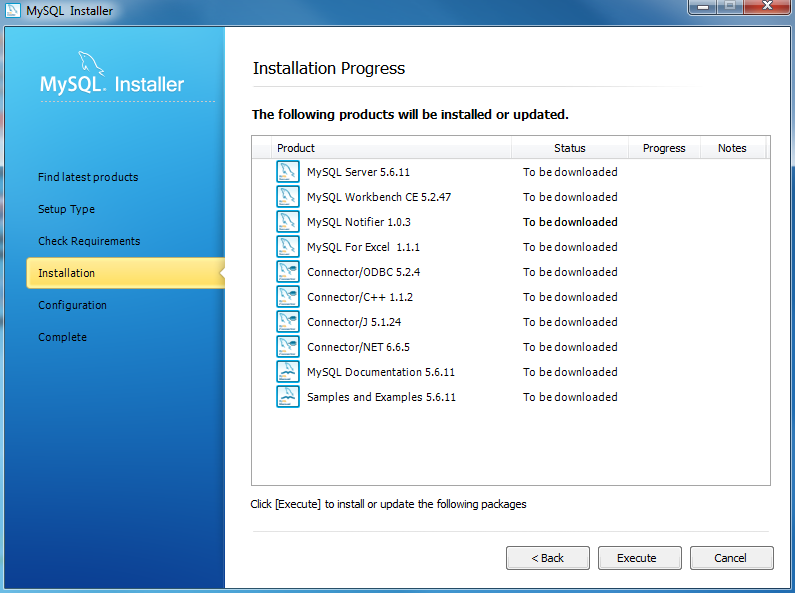
\includegraphics[width=0.6\textwidth]{/home/deepti/Desktop/my.png}                   
\caption{Installation of MySQL}
\hspace{-1.5em}
\end{figure}
\subsection*{Step 6: Change the root password }
The MySQL root user is an all-powerful account that can create and destroy databases. If you are on a shared network, it is advisable to change the default (blank) password. From the mysql> prompt, enter:\\
UPDATE mysql.user SET password=PASSWORD("my-new-password") WHERE User='root';\\
FLUSH PRIVILEGES;\\
You will be prompted for the password the next time you start the MySQL command line.\\
Enter "exit" at the mysql> prompt to stop the command line client. You should now shut down MySQL with the following command:\\
mysqladmin.exe -u root shutdown
\subsection*{Step 7: Install MySQL as Windows Service}
The easiest way to start MySQL is to add it as a Windows service. From a command prompt, enter:\\
cd mysqlbin\\
mysqld --install\\
Open the Control Panel, Administrative Tools, then Services and double-click MySQL. Set the Startup type to "Automatic" to ensure MySQL starts every time you boot your PC.\\
Alternatively, set the Startup type to "Manual" and launch MySQL whenever you choose using the command "net start mysql".



